\documentclass[12pt]{article}

%Packages
\usepackage{graphicx}
\usepackage{marginnote}
\usepackage{xcolor}
\usepackage[top=0.7cm,bottom=0cm,inner=6cm,outer=0cm,marginparwidth=6cm,marginparsep=1.1cm]{geometry}
\usepackage[light,math]{kurier}	%Font
\usepackage[T1]{fontenc}		%Font
\usepackage[hidelinks]{hyperref}
\usepackage{float}
\usepackage[utf8]{inputenc}
\usepackage{tabularx}

\author{Stefano Taillefert} % you can find my friend at github.com/Steeven9

%Various configs
\reversemarginpar			%Move margin notes to the left side
\pagenumbering{gobble}		%Remove page numbering
\definecolor{blue}{rgb}{0,0.1,0.5} %Headers
 
\begin{document}

{\centering \huge \textbf{Curriculum Vitae}}\\
\\
{\centering \huge Francesc Jordi Sacco Cremonesi}
\vspace{-0.8cm}

%Left sidebar
\marginnote{
	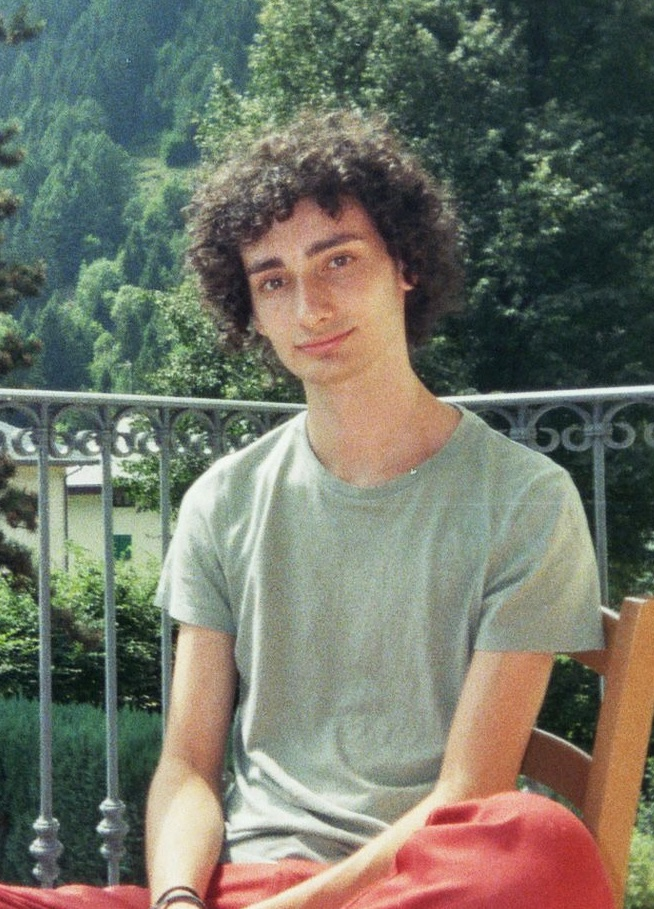
\includegraphics[width=0.7\linewidth]{img/me.jpeg}\\
	\vspace{0.5cm}
	\textbf{Francesc Jordi \\ Sacco Cremonesi}\\
    
	Via M. Carmen 4\\
	6900 Lugano (CH)\\
	\vspace{0.5cm}
	21 August 2003\\
	\vspace{0.5cm}
	% \href{tel:+come and get it}{+come and get it}\\
	% \vspace{0.5cm}
	\href{mailto:francescjordicremonesi@duck.com}{francescjordicremonesi\\@duck.com}\\
	\vspace{0.5cm}
	\href{https://github.com/sccjrd}{github.com/sccjrd}\\
}

% {\centering \huge \textbf{Curriculum Vitae}}\\
% \\
% {\centering \huge Francesc Jordi Sacco Cremonesi}
% \vspace{-0.8cm}
 
\textcolor{blue}{\section*{Education}}

\begin{table}[H]
	\begin{tabular}{ll}
		\textbf{2022 - today} & \href{https://www.usi.ch/it}{Università della Svizzera italiana}, Lugano (CH)\\
		& Bachelor of Science in Informatics\\
		\\
        \textbf{2021 - 2022} & \href{https://stmacartanscollege.ie/}{St Macartan's College}, Monaghan (IE)\\
		& Exchange Year in Ireland where I graduated\\
        & by attending the Leaving Certificate \\
        \\
		\textbf{2018 - 2021} & \href{https://www.liceodonatellipascal.edu.it/}{Liceo Scientifico B. Pascal}, Milano (IT)\\
	\end{tabular}
\end{table}
\vspace{-0.5cm}


\textcolor{blue}{\section*{Work experiences}}

\begin{table}[H]
	\begin{tabular}{ll}
        \textbf{Junior software} & July 2025 - today\\
		\textbf{engineer} & Università della Svizzera italiana, Lugano (CH)\\
        &  Developed backend automations and a simple user interface\\
        & to improve the stability and usability of MagicInfo digital\\
        & signage systems across university campuses.\\
        & Enhanced content management workflows, making it easier to\\
        & manage digital screens used for communication and events.\\
        & Continuing as a Junior Software Engineer, assisting in \\
        & the development and maintenance of front-end and back-end\\
        &software based on defined specifications.\\
        \\
        \textbf{Educator} & October 2024 - today\\
		  & \href{https://girlscodetoo.ch/schools/#}{GirlsCodeToo} (CH)\\
		& Teaching young students basic programming fundamentals \\
        & with workshops and interactive learning.\\
        \\
		\textbf{Educator and} & March 2023 - March 2026\\
		\textbf{promoter}& Università della Svizzera italiana, Lugano (CH)\\
		& Introduced students from primary to high school to basic   \\
        & programming fundamentals with interactive learning,  \\
        & such as: \href{https://www.thymio.org/}{Thymio}, Blocky VPL, \href{https://xlogo.inf.ethz.ch/release/latest/#/}{XLogo}\\
		& Helped organizing several events, coordinating groups\\
		& of collaborators while gathering the public's interest in\\
		& the projects of students and professors; helped presenting\\
		& the university's academic offers.\\
		\\
		\textbf{IT \& Multimedia} & August 2023 - June 2025\\
        \textbf{technician} & Università della Svizzera italiana, Lugano (CH)\\
		& Performed front desk activities, classroom and events \\
        & support and helped out with the implementation \\
        & of new services for the end user.\\
	\end{tabular}
\end{table}

\newpage
\textcolor{blue}{\section*{Other experiences}}

\begin{table}[H]
	\begin{tabular}{ll}
		\textbf{Volunteering} &2020\\
        & \href{https://www.mutuosoccorsomilano.it/brigata-lena-modotti/}{Brigata Lena-Modotti}, Mutuo Soccorso Milano (IT)\\ 
        & During the early stages. of the COVID-19 pandemic, we\\
        & collected food, medicines and basic necessities and handed\\
        & them out to people and families in need.
	\end{tabular}
\end{table}


\textcolor{blue}{\section*{Competences} }

\begin{table}[H]
	\begin{tabular}{ll}
		\textbf{Programming languages} & Java, C\#, C, Python, JavaScript\\
		\\
		\textbf{Web development} & HTML5, CSS3, React, Vue, Node.js\\
		& \href{https://mui.com/material-ui/}{Material-UI}, \href{https://element-plus.org/en-US/}Element$^{+}$, \href{https://tailwindcss.com/}{Tailwind}\\
        & \href{https://graphql.org/}{GraphQL}, \href{https://spring.io/projects/spring-boot}{Springboot}\\
		\\
		\textbf{Build tools} & GitLab, Jira\\
		\\
		\textbf{Other softwares} & Git, Bitbucket, MSSQL, MongoDB Compass\\
		% \\
		% \textbf{Driving licenses} & Swiss categories A, B, BE, C, CE, D1, D1E\\
	\end{tabular}
\end{table}

\textcolor{blue}{\section*{Certificates} }

\begin{table}[H]
	\begin{tabular}{ll}
        \textbf{Leaving Certificate Examination} & Issued on September 2022\\
        \textit{Scrúdú na Ardteistiméireacht} & St Macartan’s College, IE\\ 
        & Candicate Number: 157276 \\
        \\
		\textbf{B2 First  } & Issued on January 2021\\
        & Cambridge Assessment English\\ 
        & Credential ID: B3912712
		% \\
		% \textbf{Driving licenses} & Swiss categories A, B, BE, C, CE, D1, D1E\\
	\end{tabular}
\end{table}


\textcolor{blue}{\section*{Languages}}

\begin{table}[H]
	\begin{tabular}{llll}
		\textbf{Italian} & Native speaker & \hspace{1cm} \textbf{Catalan} & Native speaker\\
		\\
		\textbf{English} & C2 Leaving certificate & \hspace{1cm} \textbf{Spanish} & Native speaker\\
        & \hspace{1em}\hspace{2pt} Examination \\
	\end{tabular}
\end{table}


% \textcolor{blue}{\section*{References}}

% \begin{table}[H]
% 	\begin{tabular}{lll}
% 		% Mauro Prevostini, USI, \href{mailto:mauro.prevostini@usi.ch}{mauro.prevostini@usi.ch}\\
% 		% \\
% 	\end{tabular}
% \end{table}

\end{document}
